%#! platex %f && dvipdfmx -d 5 sample141102report
%
\documentclass[a4paper,11pt]{jarticle} 
\usepackage[dvips,usenames]{color} 
\usepackage{graphicx}
\usepackage{fancyhdr}
\usepackage{bm}  % for bmdefine
\usepackage{amsmath} % bmatrix, pmatrix
\topmargin = -5mm
\oddsidemargin = 5mm
\textwidth = 152mm
\textheight = 240mm
% \pagestyle{empty}
\pagestyle{fancyplain}
\renewcommand{\footrulewidth}{0pt}
\renewcommand{\headrulewidth}{0pt}
\bmdefine{\bx}{x}
\everymath{\displaystyle}

\begin{document}
\lhead{\small 情報システム工学科}
\rhead{\small 2014年11月2日\\宮崎イチロー}
% \cfoot{}


\centerline{\Large\gt \LaTeX を使ったレポート作成}      
\vskip 5mm
\centerline{\Large\gt 67120770 宮崎 イチロー}


\section{はじめに} 
実験したことはレポートに書いておこう.
分かりやすく簡潔に書こう.
どこまで
「分かりやすく」書けばいいかというと,
1年前の自分が読んで理解できればよい.
簡潔とは言っても,単に短いだけではだめで少なくとも
\begin{enumerate}
\item 何を実験したのか,一つ一つの手順.
\item 得られた結果(図)の説明(横軸,縦軸,プロットしている線,点の意味など)
\item 考察,自分の意見,感想
\end{enumerate}
が必要.
図を張り付けただけで説明がない場合,0点をつけられても仕方がない.
%
% このソースファイルを読んで,いろいろ数字を変更し,使い方をマスターしよう.
%
詳しい \LaTeX の使い方については,
{\tt Google} で 「{\tt latex},レポート作成」などと検索
すれば親切なページが発見できる.
「教えてもらっていない」なんていう人は $\cdots$
($\Longrightarrow$ 卒業できない.さようなら).


\section{いろいろなことができる}
\subsection{図はどうするか}
{\tt gnuplot} などで,図を作成した場合,
画面に表示している図をそのまま取り込むのではなく,
直接 {\tt eps} ファイルを生成するようにしておく.
\begin{figure}[h]
\begin{center}
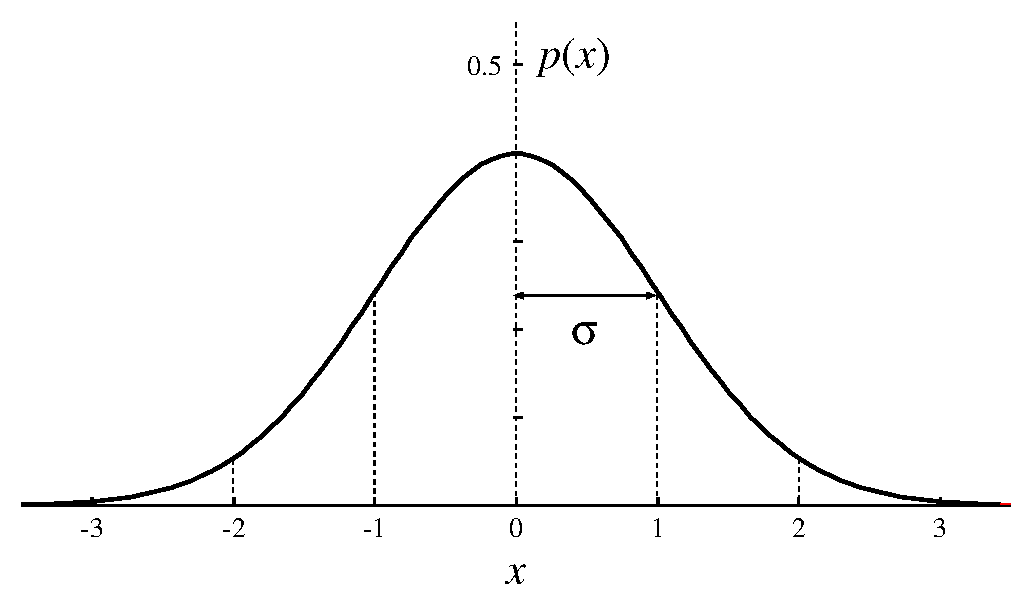
\includegraphics[width=.4\linewidth]{gauss001.eps}
\hspace*{2mm}
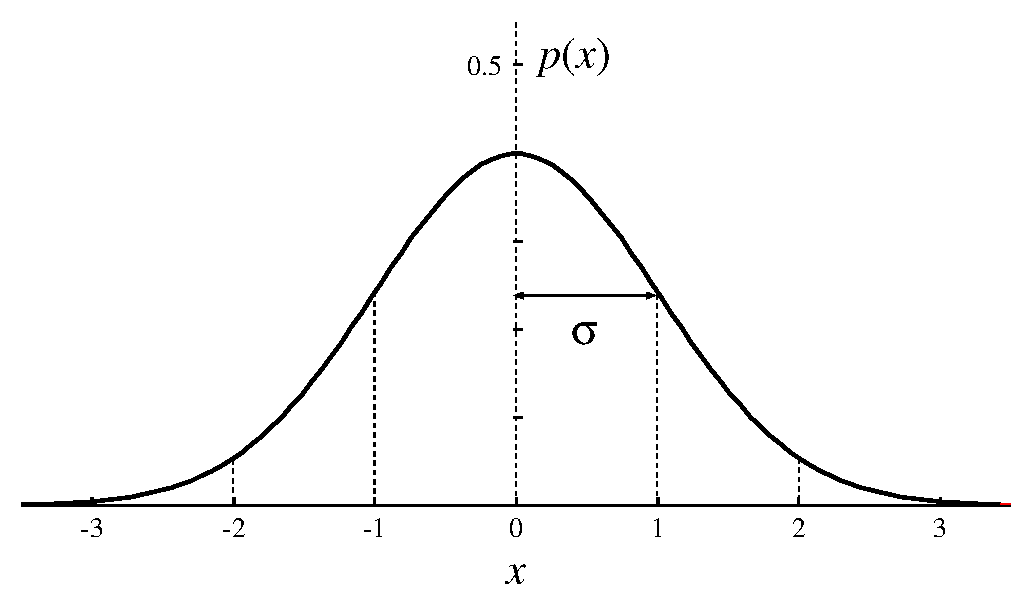
\includegraphics[width=.4\linewidth]{gauss001.eps}
\caption{平均 $0$,分散 $1$ の正規分布の確率密度関数}
\end{center}
\end{figure}

\vspace*{-10mm}

\subsection{数式は?}
普通の文章中では $ y = \sin (x)$. 式番号が必要なら
\begin{eqnarray}
a &= & \int_{-\infty}^{10}  \frac{x^2+3 \pi}{4\theta} dx \\
b & = & a + 3 \\
\bx & = & (100 \gamma, 1) \nonumber 
\end{eqnarray}

%
% これはコメント
%
%
%

\begin{thebibliography}{99}  %   文献数が10未満の時 {9}

\bibitem{amari91a}
甘利 俊一,``ニューロ多様体の情報幾何学,'' 
数理科学, no. 340, pp. 61--65, Oct, 1991.

\end{thebibliography}



\section*{付録}

\begin{figure}[htbp]
 \begin{minipage}{0.5\hsize}
  \begin{center}
   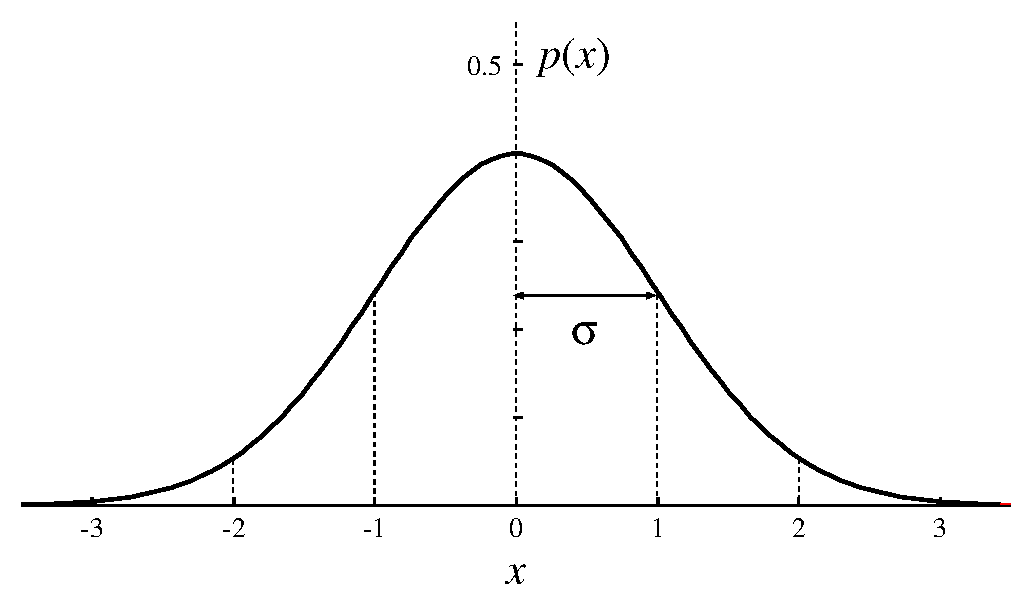
\includegraphics[width=70mm]{gauss001.eps}
  \end{center}
  \caption{1つめの図}
  \label{fig:one}
 \end{minipage}
 \begin{minipage}{0.5\hsize}
  \begin{center}
   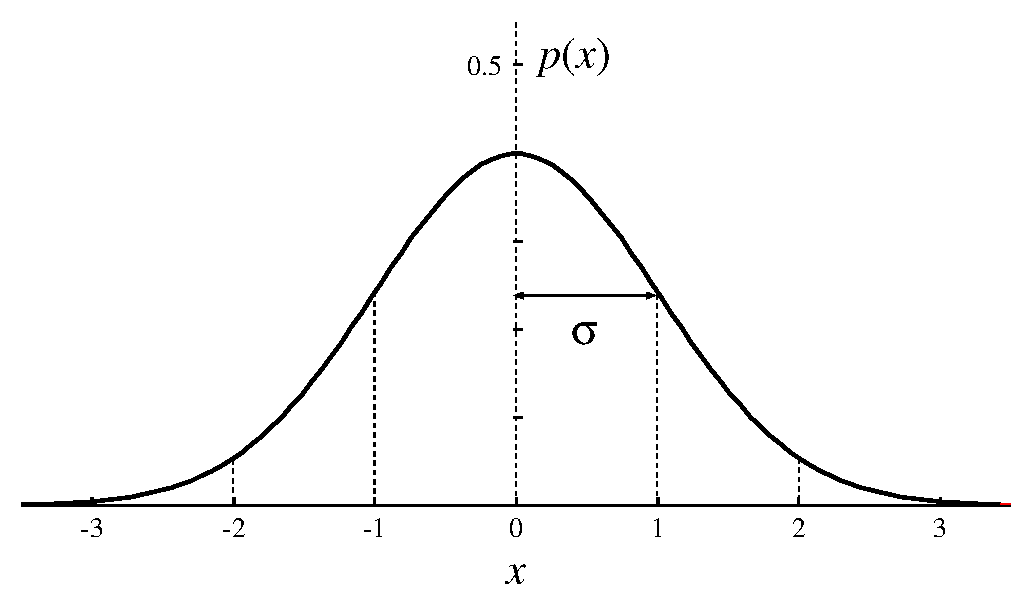
\includegraphics[width=70mm]{gauss001.eps}
  \end{center}
  \caption{2つめの図}
  \label{fig:two}
 \end{minipage}
\end{figure}


\begin{figure}[htbp]
 \begin{minipage}{0.33\hsize}
  \begin{center}
   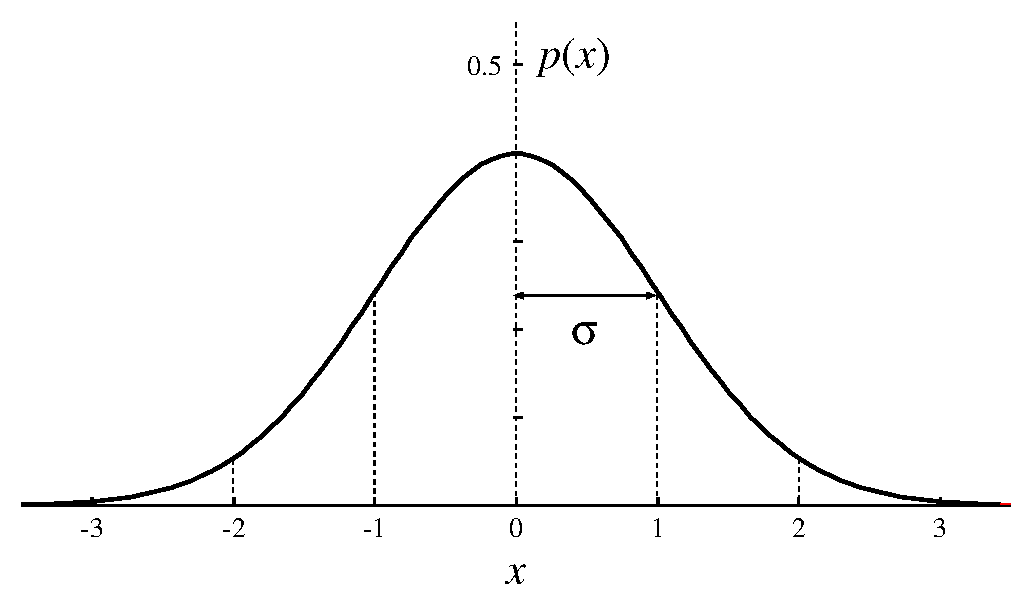
\includegraphics[width=40mm]{gauss001.eps}
  \end{center}
  \caption{3つめの図}
  \label{fig:three}
 \end{minipage}
 \begin{minipage}{0.33\hsize}
 \begin{center}
  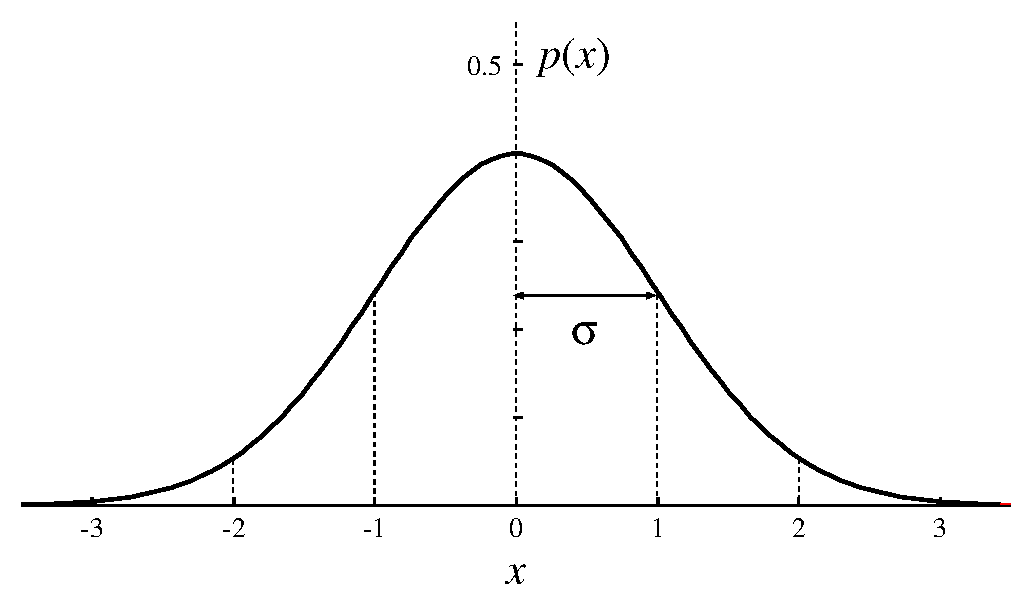
\includegraphics[width=40mm]{gauss001.eps}
 \end{center}
  \caption{4つめの図}
  \label{fig:four}
 \end{minipage}
 \begin{minipage}{0.33\hsize}
 \begin{center}
  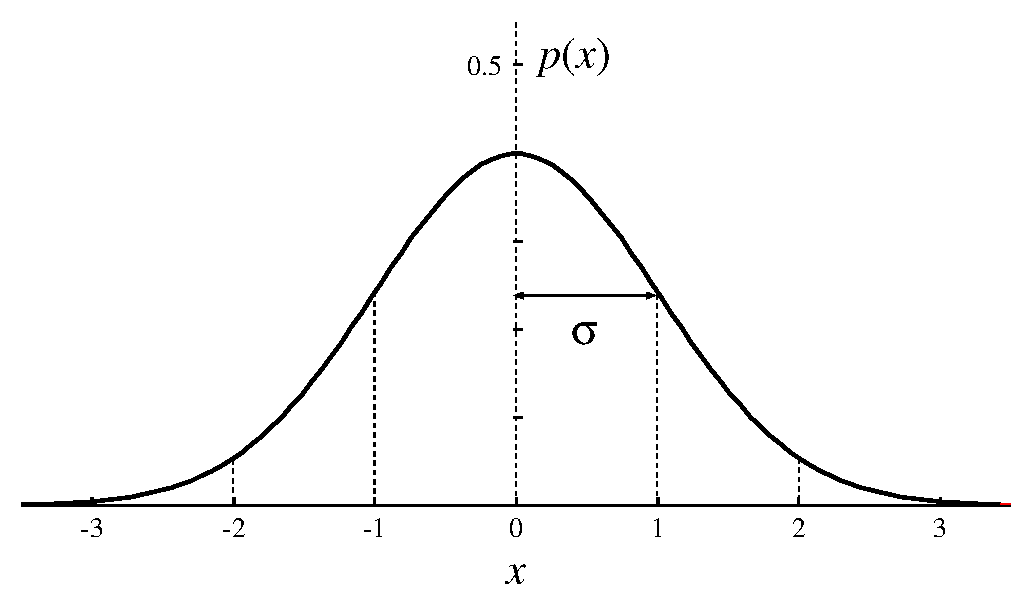
\includegraphics[width=40mm]{gauss001.eps}
 \end{center}
  \caption{5つめの図}
  \label{fig:five}
 \end{minipage}
\end{figure}


図\ref{fig:three} は左下の図です.

\lhead{}
\rhead{}


\begin{eqnarray}
\frac{dx}{dt}   & = &  - 3x \\
\frac{dx}{dt}  +2x  & = & 2t + 5 \\
x' + 2tx & = & 4t  \\
x' & = & \mathrm{e}^{-t^2} -2tx \\
x' + x & = &  \mathrm{e}^{-t} \\
x' - (\sin t) x  & = &  \sin (2t) \\
x' + x  & = &  x^2 \mathrm{e}^t \\
x' - tx   & = &  - x^3 \mathrm{e}^{-t^2}  \\
\tau \frac{dx}{dt} & = &   -x + 1 \\
\tau \frac{dx}{dt} & = &   -x + \cos t 
\end{eqnarray}

\vskip 1mm

\begin{eqnarray}
\int_1^{x} \frac{1}{x}dx   & = &  - 3 \int_0^t dt \\
\dot {\bm{x}} & = & A \bm{x} \\
\mathrm{e}^{A} & = & \sum_{k=0}^\infty \frac{A^k}{k!}
\end{eqnarray}

\begin{eqnarray}
\begin{pmatrix}
1 & 1 & 1 \\
2 & 1 & 2
\end{pmatrix}
\begin{pmatrix}
x \\
y \\
z
\end{pmatrix} 
& = &
\begin{pmatrix}
3 \\
2
\end{pmatrix}
\\
\begin{bmatrix}
1 & 1 & 1 \\
2 & 1 & 2
\end{bmatrix}
\begin{bmatrix}
x \\
y \\
z
\end{bmatrix} 
& = &
\begin{bmatrix}
3 \\
2
\end{bmatrix}
\\
A \bm{x}  & = & \bm{y}
\\
x_i & = & f(\sum_{j=1}^n w_{ij}  x_j )
\end{eqnarray}


\end{document}


